\chapter{Related work}
This chapter is about introducing CellProfiler Analyst (CPA). CPA is a first generation tool for interactive data exploration and classification of large biological image sets. 
It was first introduced in 2016 at Broad Institute of MIT and Harvard []. The following section is separated into an overview of CPA's main functionality and an exploration of its key features, Classifier and Image Gallery. This project is highly influenced by CPA and aims to improve it. The software is free and open source, available at http://www.cellprofiler.org and from GitHub under the BSD-3 license. It is available as a packaged application for
Mac OS X and Microsoft Windows and can be compiled for Linux.

\subsection{CellProfiler Analyst}
CPA is an GUI based tool. It provides easy possibilities for data exploration and classification via an interactive user interface. There are only a few comparable tools for this purpose. Most common tools are Ilastik [], CellCognition[] and WND-CHARM [].

All of these tools lack the possibility of suitable companion visualization tools, made for big datasets. Also they miss selectable classifier algorithms. Further CPA adds a big advantage to all existing tools by providing interactive object classification and image viewing.

\begin{figure}[H]
	\centering
	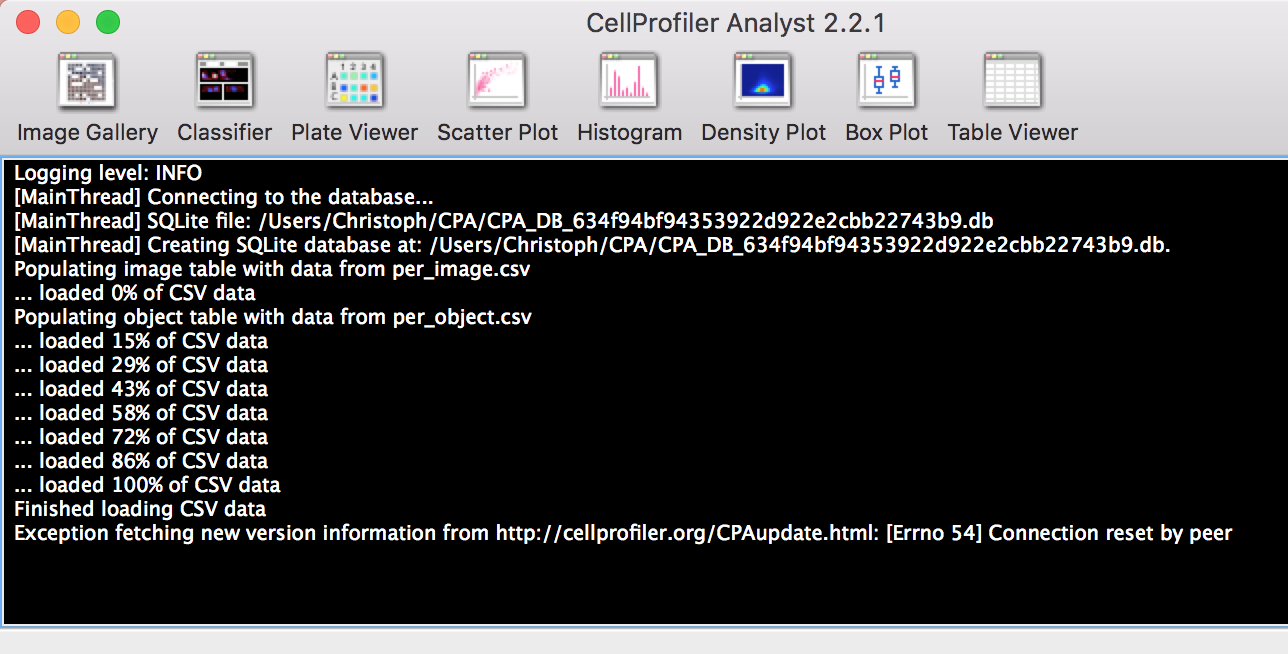
\includegraphics[width=0.8\linewidth]{bilder/related_work/cpa_main_view.png}
	\caption{CPA Main View Different Views Are Selectable} source:\cite{ReactLogo}
	\label{fig:RL}
\end{figure}

\subsection{Classifier}
Cell Profiler Analyst Classifier makes it possible to create categories and to classify cells. After fetching images from a predefined dataset it is possible to classify images by simply drag and dropping it on a category. Multi select features are also implement and enable to drag and drop multiple images at the same time. Further it is possible to add an unlimited amount of categories by clicking the add category button. After annotation is done the algorithms can be trained. Once training is done more images can fetched and the be automatically annotated by clicking the evaluate button. If results are not suffice further images can be annotated to train the algorithm in order to improve results. Different algorithms can be used to classify the uncategorized images, such as RandomForest Classifier, AdaBoost Classifier and many more.

\begin{figure}[H]
	\centering
	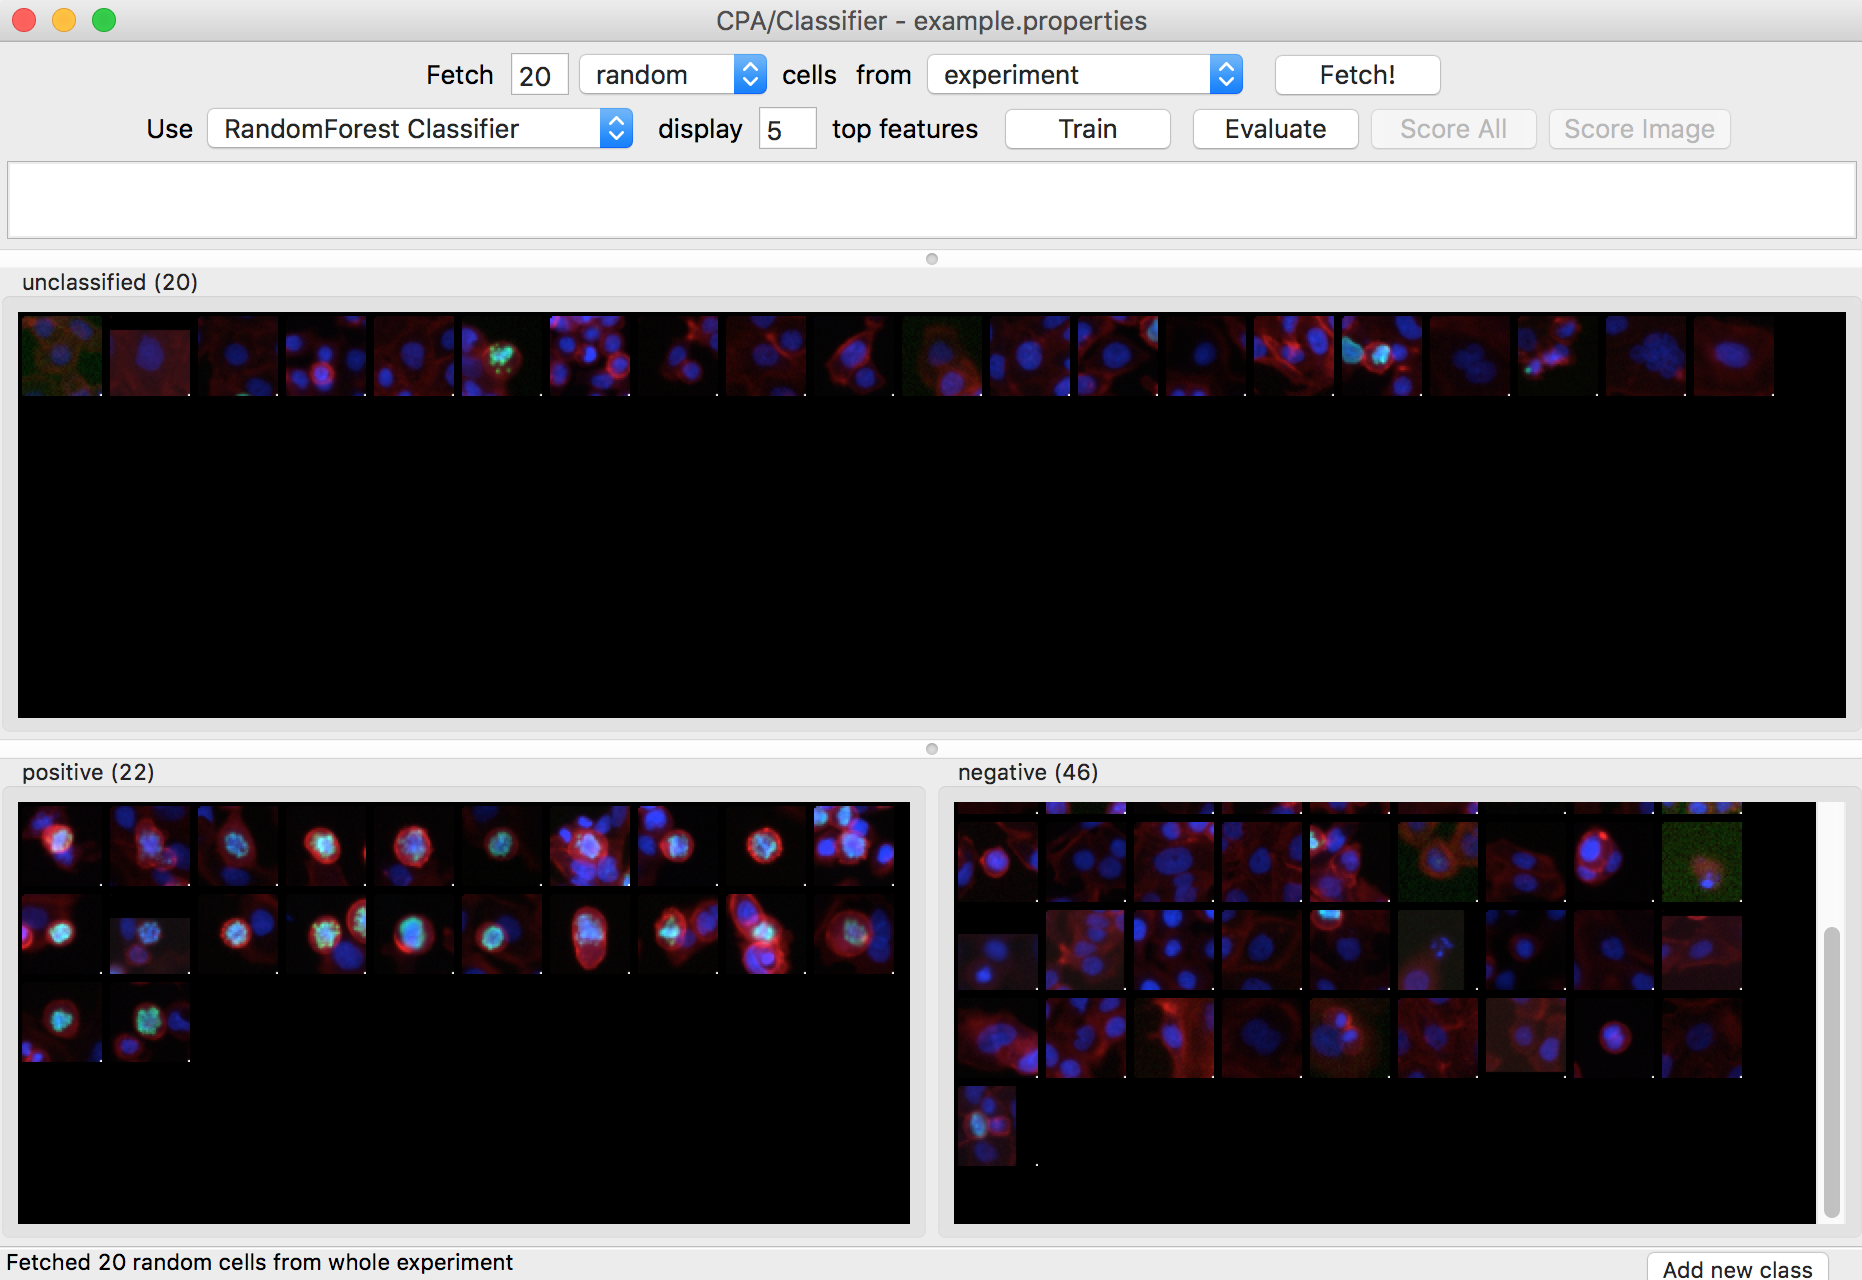
\includegraphics[width=0.7\linewidth]{bilder/related_work/classifier.png}
	\caption{CPA Main View Different Views Are Selectable} source:\cite{ReactLogo}
	\label{fig:RL}
\end{figure}


\subsection{Visualization}


In order to explore the dataset and to prediction and validation result a good visualization is needed. CPA offers different ways of displaying data and results. One simple visualization possibility is the Image Gallery in were images from the dataset can selected and be watched in their original size. Filters can be applied to only select images with a experiment specific meta data. Their are many more ways to display and explore data in CPA.

\begin{figure}[H]
	\centering
	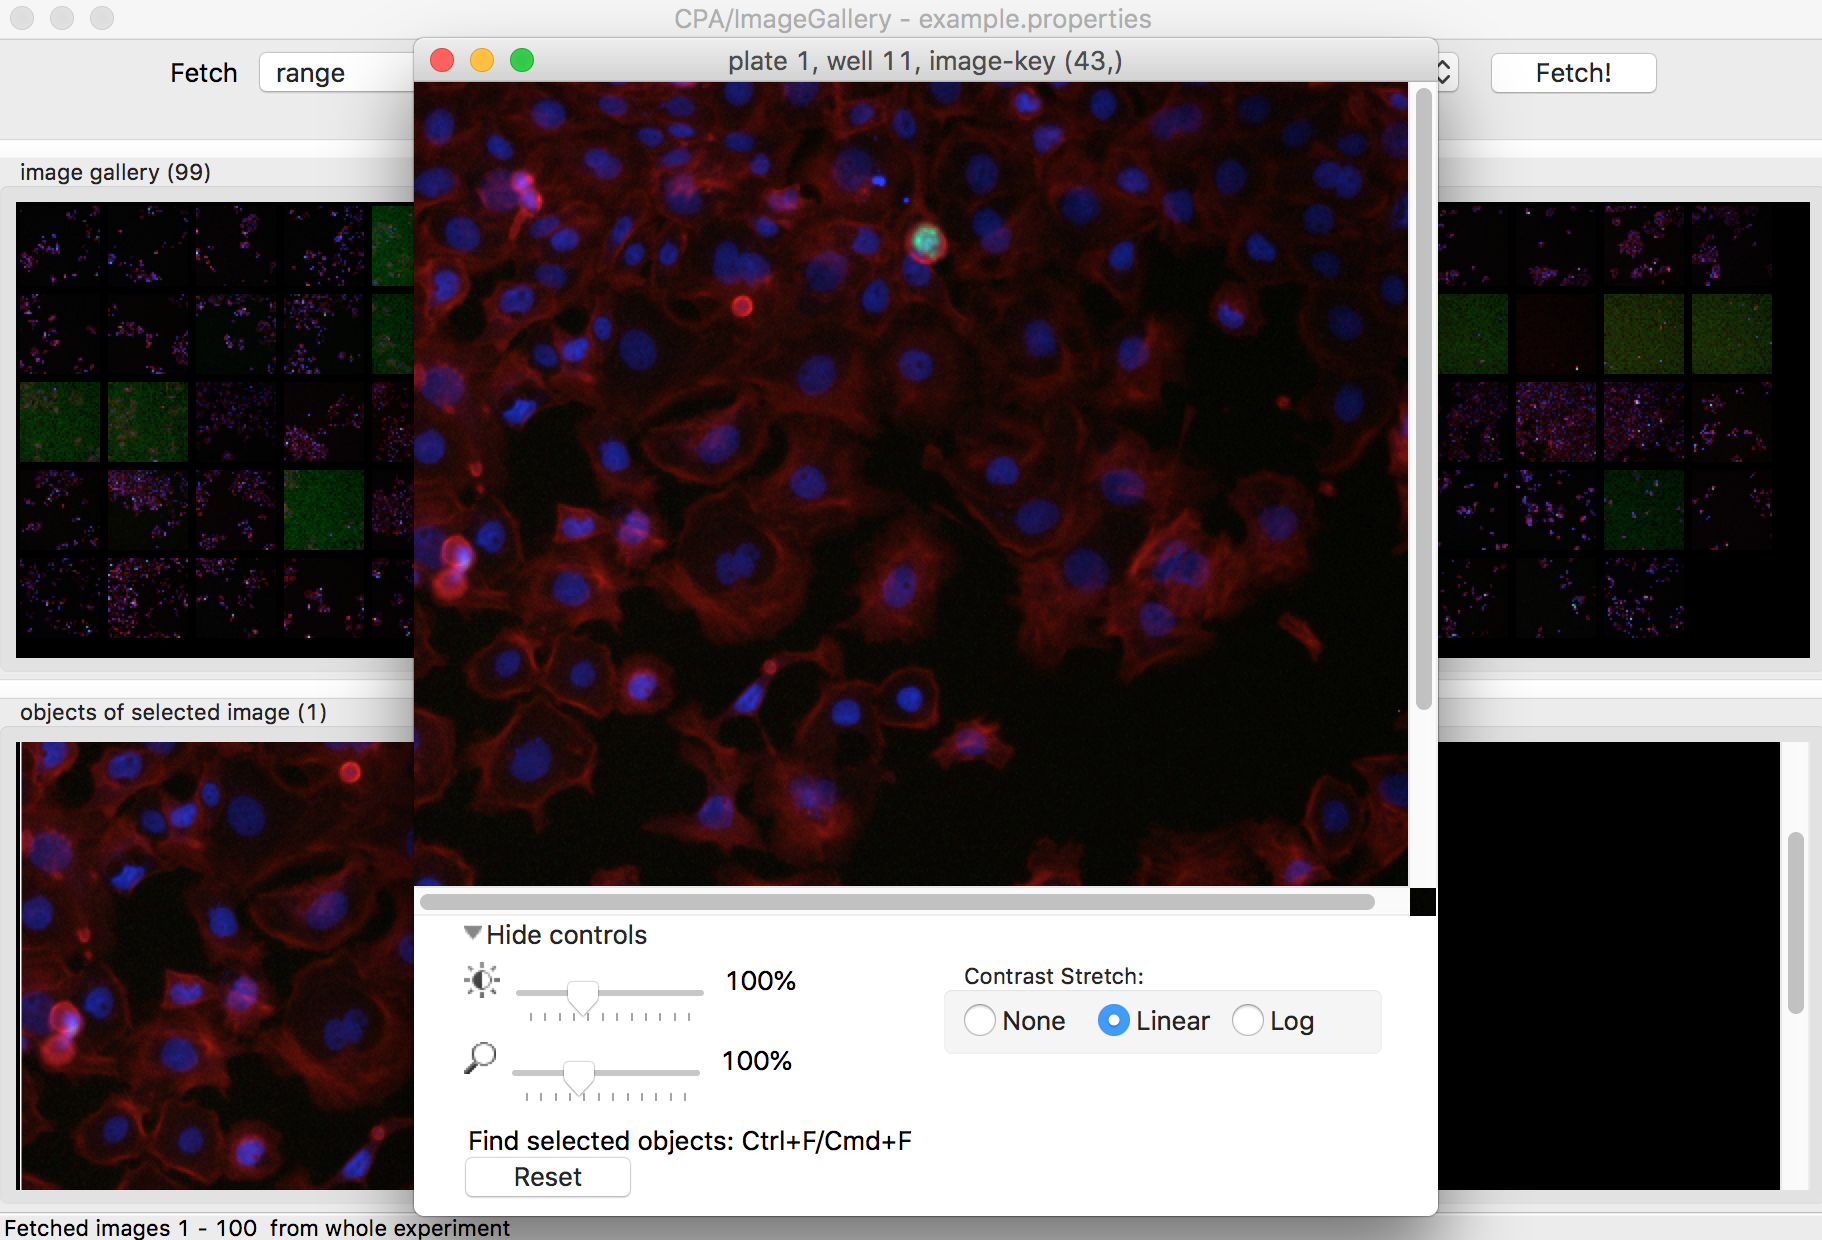
\includegraphics[width=0.7\linewidth]{bilder/related_work/visualization.png}
	\caption{CPA Main View Different Views Are Selectable} source:\cite{ReactLogo}
	\label{fig:RL}
\end{figure}


\subsection{Downsides of CPA}
To make CPA running a few steps need to be done first. 
A potential user needs to install and set up a MySQL database.
Further configuration files need to be written. The powerful user interface is also complex. Considering these things a potential user can be scared off before even using CPA. 






